\documentclass[10pt,twocolumn,letterpaper]{article}
\usepackage[margin=0.65in,columnsep=0.24in]{geometry}
\usepackage[T1]{fontenc}
\usepackage{mathptmx}
\usepackage{microtype}
\usepackage{amsmath}
\usepackage{booktabs,tabularx}
\usepackage{xcolor}
\usepackage{enumitem}
\usepackage{titlesec}
\usepackage{tikz}
\usetikzlibrary{arrows.meta}
\usepackage[font=small,labelfont=bf,skip=3pt]{caption}
\usepackage[hidelinks]{hyperref}

\titleformat*{\section}{\normalsize\bfseries}
\titleformat*{\subsection}{\small\bfseries}
\titlespacing*{\section}{0pt}{5pt plus 2pt minus 1pt}{2pt plus 1pt}
\titlespacing*{\subsection}{0pt}{3pt plus 1pt}{1pt}
\setlist{nosep,leftmargin=*}
\setlength{\textfloatsep}{6pt plus 2pt minus 2pt}
\setlength{\floatsep}{6pt plus 2pt minus 2pt}
\setlength{\abovedisplayskip}{3pt plus 1pt}
\setlength{\belowdisplayskip}{3pt plus 1pt}

% Placeholders that must be replaced with real values before submission.
\newcommand{\tbd}[1][TBD]{\textcolor{red}{\textbf{[#1]}}}
\newcommand{\para}[1]{\textbf{#1}\hspace{0.4em}}

\begin{document}

\twocolumn[{%
\begin{center}
{\Large\bfseries Content- and Load-Aware Routing of Text and Multimodal Requests\\[1pt]
Across Heterogeneous CPU and Laptop Endpoints}\\[4pt]
{\small CSE 291A Fall 2026 \textbullet{} Option 3: Adaptive Routing Across Heterogeneous Machines \textbullet{} Phase 1 Report}\\[2pt]
{\small Jason Zhu, Fengfei Yu, Hanyu Li, Mengyao Ma, Zavier Zhao}\\[1pt]
{\small\texttt{\{jaz019, fey006, hal209, mem032, zhz214\}@ucsd.edu}}
\end{center}\vspace{4pt}}]

\section{Problem and Research Question}
Cloud CPU instances and laptops differ in compute, memory bandwidth, capacity,
and network distance. Qwen3.5~\cite{qwen35} (natively image--text-to-text;
dense 0.8B--27B and MoE \mbox{35B-A3B}) also offers tiers that trade quality for cost.
Serving a request therefore couples three per-request decisions (\emph{which
tier}, \emph{which machine}, and \emph{when}) with a slower one: \emph{which
models} each machine keeps loaded. Phase~1 measures the differences, and
Phase~2 derives the router from them.

\para{Core question.} \emph{When should a text or image request run on each
machine and model tier, given its content and shape, the fleet's load relative
to capacity, and the cost of moving the request and its context?}
\begin{itemize}
\item[\textbf{H1}] \emph{Shape dependence.} Prefill (compute-bound), decode
(bandwidth-bound), and vision encoding scale differently across ISAs, core
counts, and Apple-Silicon GPUs, so the best idle device depends on request
shape.
\item[\textbf{H2}] \emph{Content predictability.} Cheap prompt features
predict the smallest adequate tier and the output length well enough to pay
for the decision.
\item[\textbf{H3}] \emph{Capacity regimes.} Below capacity, placement
dominates. Above it, ordering, batching, and model residency matter more, and
speed-oblivious policies misroute~\cite{harchol}.
\item[\textbf{H4}] \emph{Communication.} Transfer is negligible for text inside
AWS but not for images sent over the WAN to laptops.
\end{itemize}

\section{Environment and Endpoints}
\begin{table}[!htb]
\centering\footnotesize
\caption{Endpoints. A--C and R share one AWS AZ; laptops are off-cloud.
``Can host'' lists memory-feasible Q4 models, loaded on demand; the laptop
range depends on RAM (16\,GB: up to 9B; 48\,GB: up to 35B-A3B). Instance types
are pending an eligibility check.}
\label{tab:endpoints}
\begin{tabularx}{\columnwidth}{@{}lXl@{}}
\toprule
ID & Hardware & Can host \\
\midrule
A & \texttt{c7g.xlarge}: Graviton3, 4 cores, 8\,GB & 0.8B--4B \\
B & \texttt{c7g.2xlarge}: Graviton3, 8 cores, 16\,GB & 0.8B--9B \\
C & \texttt{c7i.2xlarge}: Xeon SPR, 4C/8T, 16\,GB, AMX & 0.8B--9B \\
L & 5 MacBook Pro/Air: Apple Silicon (Metal), 16--48\,GB & 0.8B--35B-A3B \\
R & \texttt{c7g.medium}: router + load generator & -- \\
\bottomrule
\end{tabularx}
\end{table}

\para{Core and extended study.} The core study follows the option
specification: three AWS CPU instance types and the router in one Region, over
private IPs. Each pair changes one factor. A vs.\ B varies cores and memory on
one ISA. B vs.\ C varies the ISA (Arm Neoverse-V1 vs.\ x86 with AVX-512/AMX) at
equal vCPUs and memory; C has half of B's physical cores because an x86 vCPU
is a hyperthread. The extended study adds five Apple-Silicon MacBooks (Metal
GPU, unified memory), reached over the WAN through a WireGuard tunnel, which is
a second communication regime.

\para{Runtime and models.} Every device runs one pinned llama.cpp
release~\cite{llamacpp} (\texttt{llama-server}; images via \texttt{mmproj}),
built natively per backend (Arm, x86, Metal), with identical SHA-256-verified
GGUF files and thinking mode off. Devices are \emph{not} bound to one model: every GGUF that
fits is pre-staged on disk, and a per-device agent starts or stops one
\texttt{llama-server} per resident model at the router's request.

\para{Confounder control.} Hardware comparisons use matched models (0.8B and
2B at Q4\_K\_M on every device); each device's best practical configuration is
reported separately. Results that change the tier are always
reported with answer quality, so gains from a smaller model are never credited
to routing.

\section{Workloads and Metrics}
\para{Requests.} Text: \textbf{T1} short chat; \textbf{T2} prefill-heavy
(2--8K-token document, short answer); \textbf{T3} decode-heavy; \textbf{T4}
multi-step agent sessions with accumulating context and tool delays. Image:
\textbf{M1} single image at three resolutions; \textbf{M2} chart or document;
\textbf{M3} multi-image. Prompts come from public chat traces and from
benchmarks with programmatic checks (GSM8K, MMLU; ChartQA, TextVQA), whose
varying difficulty yields tier labels (E5).

\para{Load.} Open-loop Poisson and on/off bursty arrivals are replayed from
fixed seeds at offered loads $\rho=0.5$--$1.5$ of measured fleet capacity,
covering both regimes. Policies are tuned on dev mixes and evaluated on
held-out mixes with different text:image ratios and lengths. Performance runs
fix output length (\texttt{n\_predict}, \texttt{ignore\_eos}); quality runs
terminate naturally.

\para{Metrics.} Per request: TTFT, TPOT, end-to-end latency, queueing delay,
chosen (device, tier), correctness, and status (timeouts and rejections are
kept). Per device at 1\,Hz: CPU/GPU utilization, memory, slot occupancy, and
resident models. Aggregates: throughput, p50/p99 TTFT and TPOT, SLO
attainment, accuracy vs.\ always-largest, network bytes, decision latency, and
swap time. Versions are pinned, and runs are repeated at least three times
(median, bootstrap 95\% CI). Cold and warm start are reported separately, and
laptops run on AC power in a fixed performance mode.

\section{Phase 1 Measurements}
\begin{itemize}
\item[\textbf{E1}] \emph{Isolated profiles:} device $\times$ model $\times$
quant $\times$ lengths $\times$ image resolution $\rightarrow$ prefill rate,
TPOT vs.\ context, vision-encode time, and memory.
\item[\textbf{E2}] \emph{Load curves:} slots 1--8 and arrival rate up to
saturation $\rightarrow$ latency vs.\ load, capacity, and batching gain.
\item[\textbf{E3}] \emph{Communication and state:} RTT and bandwidth (intra-AZ
vs.\ WAN), transfer time vs.\ payload, warm vs.\ switched sessions, and router
overhead.
\item[\textbf{E4}] \emph{Model lifecycle:} load and unload time per (device,
model), and co-location interference.
\item[\textbf{E5}] \emph{Tier labels:} each dev prompt on each tier
$\rightarrow$ the smallest passing tier and the output length.
\end{itemize}
E1--E4 calibrate the cost model and the crossover maps (the best device per
class, idle vs.\ loaded); E5 trains the tier selector.

\section{Phase 2: Router Architecture}
\begin{figure}[!t]
\centering
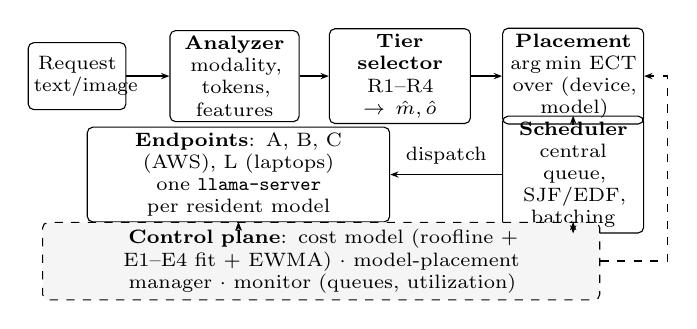
\begin{tikzpicture}[font=\scriptsize,
  b/.style={draw,rounded corners=2pt,align=center,inner sep=2pt,minimum height=0.85cm},
  c/.style={draw,dashed,rounded corners=2pt,align=center,inner sep=2.5pt,fill=black!4},
  a/.style={-{Stealth[length=3pt]},semithick},
  d/.style={{Stealth[length=3pt]}-{Stealth[length=3pt]},semithick,dashed}]
\node[b,text width=1.1cm]  (req) at (0,0) {Request\\text/image};
\node[b,text width=1.5cm]  (ana) at (2.0,0) {\textbf{Analyzer}\\modality, tokens, features};
\node[b,text width=1.65cm] (tier) at (4.1,0) {\textbf{Tier selector}\\R1--R4 $\rightarrow \hat m, \hat o$};
\node[b,text width=1.65cm] (plc) at (6.3,0) {\textbf{Placement}\\$\arg\min$ ECT over (device, model)};
\node[b,text width=1.65cm] (sch) at (6.3,-1.25) {\textbf{Scheduler}\\central queue, SJF/EDF, batching};
\node[b,text width=3.7cm]  (ep) at (2.05,-1.25) {\textbf{Endpoints}: A, B, C (AWS), L (laptops)\\one \texttt{llama-server} per resident model};
\node[c,text width=6.9cm]  (ctl) at (3.1,-2.35) {\textbf{Control plane}: cost model (roofline + E1--E4 fit + EWMA)
  $\cdot$ model-placement manager $\cdot$ monitor (queues, utilization)};
\draw[a] (req) -- (ana);
\draw[a] (ana) -- (tier);
\draw[a] (tier) -- (plc);
\draw[a] (plc) -- (sch);
\draw[a] (sch) -- node[above]{dispatch} (ep);
\draw[d] (ep.south) -- (ep.south |- ctl.north);
\draw[d] (sch.south) -- (sch.south |- ctl.north);
\draw[-{Stealth[length=3pt]},semithick,dashed] (ctl.east) -- (7.5,-2.35) |- (plc.east);
\end{tikzpicture}
\caption{Router architecture. Solid arrows: per-request data plane. Dashed:
control plane (model load/unload, metrics, queue state, cost updates). The
placement manager changes which models are resident on each device.}
\label{fig:arch}
\end{figure}
\para{Expected performance from model configuration.} The router
(Fig.~\ref{fig:arch}) needs a cost model. For model $m$ on device
$i$, a roofline estimate gives prefill time and decode time per token:
\begin{align}
P_{i,m}(p) &\approx 2N_m p\,/\,(\eta^{c}_i F_i),\\
\mathrm{TPOT}_{i,m}(b) &\approx \max\{(S_m+bK_m)/(\eta^{m}_i \beta_i),\; 2bN_m/(\eta^{c}_i F_i)\}.
\end{align}
$p$ is the number of prompt tokens and $b$ the decode batch size. $N_m$ is the
number of active parameters (3B for 35B-A3B), $S_m$ the quantized weight bytes,
and $K_m$ the per-sequence KV/state bytes read per step. $F_i$ and $\beta_i$
are peak FLOP/s and memory bandwidth. The efficiencies $\eta$ are fitted from
E1--E2 and EWMA-corrected online, and vision encoding $V_i(v)$ is fitted in
image tokens $v$. The decode term shows that batching is nearly free until the
device becomes compute-bound. The estimated completion time of request $r$ on
$(i,m)$ is
\begin{equation}
\begin{aligned}
\mathrm{ECT}_{i,m}(r) ={}& W_i + V_i(v_r) + P_{i,m}(p_r) + \hat{o}_r\,\mathrm{TPOT}_{i,m}(b_i)\\
&+ \mathrm{RTT}_i + s_r/\mathrm{BW}_i + C_i(r) + L_{i,m},
\end{aligned}
\end{equation}
where $W_i$ is the work queued on $i$, $\hat{o}_r$ the predicted output length,
and $s_r$ the payload size. $C_i$ is the re-prefill penalty when the session's
state is elsewhere, and $L_{i,m}$ is the load time when $m$ is not resident.

\para{Content-based tier selection (the core decision).} The selector predicts
the smallest adequate tier $\hat m(r)$ and an output-length bucket $\hat o_r$,
using mechanisms of increasing cost:
\begin{itemize}
\item[\textbf{R1}] \emph{Rules:} modality, length thresholds, and regex cues
(code, math, ``prove''/``explain'').
\item[\textbf{R2}] \emph{Classic NLP:} TF-IDF and hand-crafted features
(length, math/code density, question type) fed to logistic regression or
boosted trees; sub-millisecond on a CPU.
\item[\textbf{R3}] \emph{Tiny-LM router:} Qwen3.5-0.8B scoring a one-token
label, or a small fine-tuned encoder (cf.\ RouteLLM~\cite{routellm}). More
accurate, but its prefill is charged to TTFT.
\item[\textbf{R4}] \emph{Cascade:} R2 decides, and R3 is called only when R2's
confidence is below $\theta$ (cf.\ FrugalGPT~\cite{frugalgpt}).
\end{itemize}
All four are trained on E5 labels and judged on tier accuracy, end-task
quality, and decision latency relative to service time.

\para{Scheduling below and above capacity.} Below capacity, each request goes
greedily to $\arg\min_{(i,m)}\mathrm{ECT}$ over feasible pairs (tier at least
$\hat m$, fits in memory), so a slow idle device is used only if it finishes
sooner. Above capacity or during bursts, requests wait in a central router
queue and are bound to an endpoint only when a slot frees (late binding). The
queue is ordered by predicted size with aging (SJF) or by deadline (EDF).
Small same-tier requests are batched, a request may be downgraded within an
explicit quality budget, and admission control sheds load; rejections count
as failures.

\para{Dynamic model placement.} Every $\Delta$ seconds the placement manager
re-plans which models are resident on each device from per-tier demand
forecasts (EWMA arrival rates), within memory limits. For example, it can start
an extra 0.8B server on B or a laptop when small requests surge, so that they
can be batched. It changes residency only when the expected gain over the
planning horizon exceeds the measured load time and co-location interference
(E4), with hysteresis against thrashing.

\para{Baselines and evaluation.} Baselines: always-$i$, round-robin,
least-outstanding-requests, weighted round-robin tuned on dev, static
device-to-model binding, and always-largest (the quality reference). We
evaluate steady and bursty arrivals across $\rho$ on held-out mixes, with the
fastest device idle and busy. We ablate R1--R4, analytic vs.\ measured cost,
oracle vs.\ predicted tier and length, the scheduling policy, and dynamic
vs.\ static placement. A simple policy sufficing is a valid outcome.

\para{Scope and risks.} Must-have: the cost model, ECT placement, R1--R2, both
load regimes, and all baselines. Stretch: R3--R4 and dynamic placement. Risks:
(1)~Qwen3.5 vision in llama.cpp is not yet verified on every backend.
(2)~Laptop/WAN variability (repeated runs, reported variance). (3)~Budget: the team's $5\times\$25=\$125$ buys about 150\,h of
A+B+C+R at about \$0.83/h (to be confirmed); we develop on laptops,
auto-shut down instances, and set billing alarms.

{\footnotesize
\begin{thebibliography}{9}\setlength{\itemsep}{0pt}
\bibitem{llamacpp} llama.cpp. \url{https://github.com/ggml-org/llama.cpp}
\bibitem{qwen35} Qwen Team. Qwen3.5 model collection.
\url{https://huggingface.co/collections/Qwen/qwen35}
\bibitem{harchol} M.~Harchol-Balter. \emph{Performance Modeling and Design of
Computer Systems}. Cambridge Univ.\ Press, 2013.
\bibitem{routellm} I.~Ong et al. RouteLLM: Learning to route LLMs with
preference data. arXiv:2406.18665, 2024.
\bibitem{frugalgpt} L.~Chen, M.~Zaharia, J.~Zou. FrugalGPT. arXiv:2305.05176,
2023.
\end{thebibliography}}

\appendix
\section*{Appendix A: Timeline and Milestones}
{\footnotesize\setlength{\tabcolsep}{3pt}\renewcommand{\arraystretch}{1.05}
\noindent\begin{tabularx}{\columnwidth}{@{}>{\raggedright\arraybackslash}p{0.8in}>{\raggedright\arraybackslash}X@{}}
\toprule
Stage & Work and milestones (Thanksgiving, Nov 26--29, is buffer) \\
\midrule
\textbf{1. Environment setup}\newline Nov 3--8 &
Confirm eligibility and quota; provisioning scripts; pinned llama.cpp builds;
GGUF/\texttt{mmproj} on every device; WAN tunnel; model agent; load generator
and logging; pass-through router.
\textbf{M0 (Nov 4):} Phase~1 report. \textbf{M1 (Nov 8):} every device serves
0.8B text and image requests through the router. \\
\addlinespace[2pt]
\textbf{2. Config.\ testing \& expectation setup}\newline Nov 6--18 &
E1--E5 sweeps (models, quantizations, lengths, image resolutions, load,
network, model lifecycle); fit roofline efficiencies; collect tier labels;
freeze dev/held-out traces. \textbf{M2 (Nov 18):} calibrated cost model,
labeled dev set. \\
\addlinespace[2pt]
\textbf{3. Router development}\newline Nov 16--28 &
Baselines; ECT placement; R1--R2, then R3--R4; central-queue scheduler;
placement manager (stretch); decision-latency microbenchmarks.
\textbf{M3 (Nov 25):} router and baselines run end-to-end on dev mixes. \\
\addlinespace[2pt]
\textbf{4. Experiments \& analysis}\newline Nov 25--Dec 10 &
Held-out runs across $\rho$ (steady and bursty; fastest device idle and busy);
ablations; repeated runs with CIs; failure analysis; report and artifacts.
\textbf{M4 (Dec 5):} all runs complete. \textbf{M5 (Dec 10):} final report. \\
\bottomrule
\end{tabularx}\par}

\end{document}
